\chapter{Exportando dados}

InVesalius allows to export data in different formats, such as OBJ, STL and others, to be used in other software.

Menu to export data is located in the left panel of InVesalius,
inside item \textbf{4. Export data}. If the menu is not visible, double-click with \textbf{left} mouse button
to expand the item. Figure \ref{fig:data_export} exhibit this menu.

\begin{figure}[!htb]
\centering
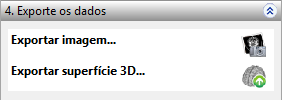
\includegraphics[scale=0.8]{painel_data_export_pt.png}
\caption{Menu to export data}
\label{fig:data_export}
\end{figure}

\section{Surface}

To export a surface, select it from the data menu as shown in
figure \ref{fig:data_export_selection}.

\newpage

\begin{figure}[!htb]
\centering
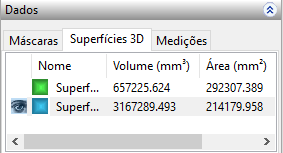
\includegraphics[scale=0.7]{painel_data_export_selection_pt.png}
\caption{Select surface to be exported}
\label{fig:data_export_selection}
\end{figure}

Next, click on the icon shown in figure \ref{fig:surface_export_original}.

\begin{figure}[!htb]
\centering

\includegraphics[scale=0.2]{surface_export_original}
\caption{Shortcut to export surface}
\label{fig:surface_export_original}
\end{figure}

In the correspondent window (figure \ref{fig:export_data_window}), tyoe the file name and
select the desired exported format. Finally, click \textbf{Save}.


\begin{figure}[!htb]
\centering
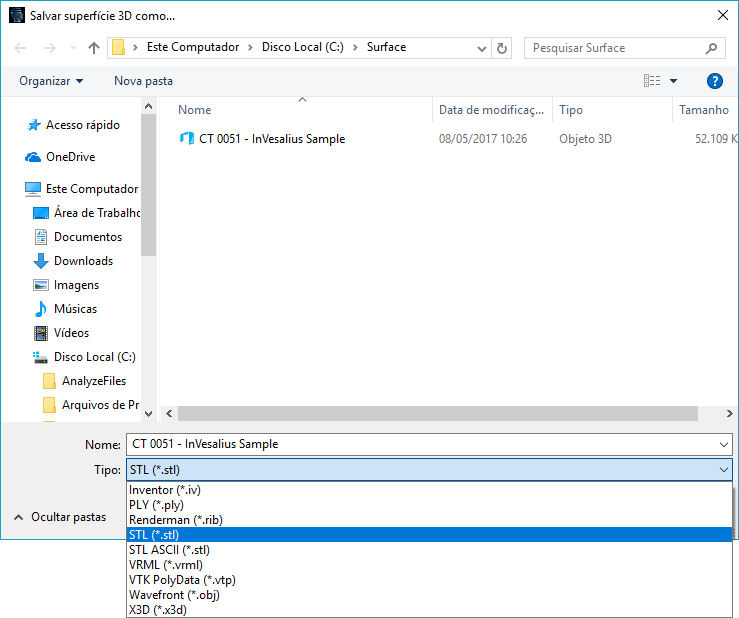
\includegraphics[scale=0.4]{export_surface.png}
\caption{Window to export surface}
\label{fig:export_data_window}
\end{figure}

Files formats avaiable for exportation are listed in table
\ref{tab:files_export_list}:

\begin{table}[h]
\centering
\caption{File formats exported by InVesalius}
\begin{tabular}{lcc}\\
\hline % este comando coloca uma linha na tabela
Format & Extension\\
\hline
\hline
Inventor & .iv\\
Polygon File Format & .ply\\
Renderman & .rib\\
Stereolithography (formato binário)& .stl\\
Stereolithography (formato ASCII) & .stl\\
VRML & .vrml\\
VTK PolyData & .vtp\\
Wavefront & .obj\\
\hline
\end{tabular}
\label{tab:files_export_list}
\end{table} 


\section{Image}

Images exhibited in any orientation (axial, coronal,
sagittal and 3D) can be exported. To do so, click with mouse \textbf{left} button on the shortcut
shown in figure \ref{fig:menu_save_image_window} and select the sub-window related to the target
image to be exported.

\begin{figure}[!htb]
\centering
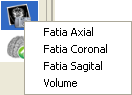
\includegraphics[scale=0.5]{menu_save_image_window_pt.png}
\caption{Menu to export images}
\label{fig:menu_save_image_window}
\end{figure}

On the windown shown (figure \ref{fig:save_image_window}), select the desired file cormat and click
on the button \textbf{Save}.

\begin{figure}[!htb]
\centering
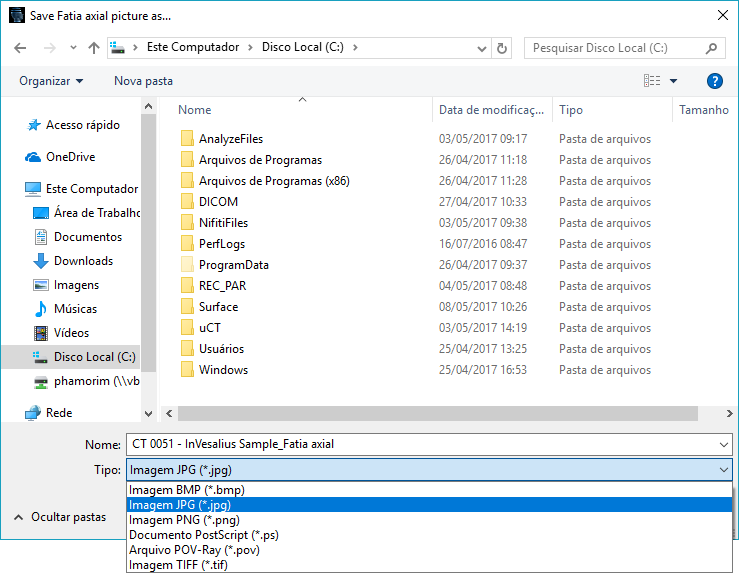
\includegraphics[scale=0.4]{export_bmp_pt.png}
\caption{Window to export images}
\label{fig:save_image_window}
\end{figure}
